\documentclass[12pt,titlepage]{article}
\usepackage[margin=1.25in]{geometry}
\usepackage{graphicx,amsmath,minted}

%% Variables definition
\newcommand{\vSubject}{Object Oriented Programming}
\newcommand{\vSubtitle}{Encapsulation}
\newcommand{\vName}{Dicha Zelianivan Arkana}
\newcommand{\vNIM}{2241720002}
\newcommand{\vClass}{2i}
\newcommand{\vDepartment}{Information Technology}
\newcommand{\vStudyProgram}{D4 Informatics Engineering}

%% [START] Tikz related stuff
\usepackage{tikz}
\usetikzlibrary{svg.path,calc,shapes.geometric,shapes.misc}
\tikzstyle{terminator} = [rectangle, draw, text centered, rounded corners = 1em, minimum height=2em]
\tikzstyle{preparation} = [chamfered rectangle, chamfered rectangle sep=0.75em, draw, text centered, minimum height = 2em]
\tikzstyle{process} = [rectangle, draw, text centered, minimum height=2em]
\tikzstyle{decision} = [diamond, aspect=2, draw, text centered, minimum height=2em]
\tikzstyle{data}=[trapezium, draw, text centered, trapezium left angle=60, trapezium right angle=120, minimum height=2em]
\tikzstyle{connector} = [line width=0.25mm,->]
%% [END] Tikz related stuff

%% [START] Fancy header related stuff
\usepackage{fancyhdr}
\pagestyle{fancy}
\setlength{\headheight}{15pt} % compensate fancyhdr style
\fancyhead{}
\fancyfoot{}
\fancyfoot[L]{\thepage}
\fancyfoot[R]{\textit{\vSubject - \vSubtitle}}
\renewcommand{\footrulewidth}{0.4pt}% default is 0pt, overline for footer
%% [END] Fancy header related stuff

%% [START] Custom tabular command related stuff
\usepackage{tabularx}
\newcommand{\details}[2]{
    #1 & #2  \\
}
%% [END] Custom tabular command related stuff

%% [START] Figure related stuff
\newcommand{\image}[3][1]{
    \begin{figure}[h]
        \centering
        \includegraphics[#1]{#2}
        \caption{#3}
        \label{#3}
    \end{figure}
}
%% [END] Figure related stuff

\begin{document}
\begin{titlepage}
    \centering
    \vfill
    {\bfseries\LARGE
        \vSubject\\
        \vskip0.25cm
        \vSubtitle
    }
    \vfill
    
\includegraphics[width=6cm]{images/polinema-logo.png}
    \vfill
    {
        \textbf{Name}\\
        \vName\\
        \vskip0.5cm
        \textbf{NIM}\\
        \vNIM\\
        \vskip0.5cm
        \textbf{Class}\\
        \vClass\\
        \vskip0.5cm
        \textbf{Department}\\
        \vDepartment\\
        \vskip0.5cm
        \textbf{Study Program}\\
        \vStudyProgram
    }
\end{titlepage}

\section{Practicum - Encapsulation}
\subsection{Questions}
\begin{enumerate}
    \item {
        Inside the class \texttt{TestMobil}, when we add the speed for the first time, why did we get
        a warning "The speed can't be added because the car is off"?

        Because it's illogical to add speed when the car is off. We've added a validation rule to prevent this
        from happening.
    }
    \item {
        Why does the attribute \texttt{speed} and \texttt{contactOn} have the \texttt{private} access modifier?

        Because we want to encapsulate the data so that it can only be accessed from within the class. We don't want
        the data to be accessed from outside the class because we can't guarantee that the data will be valid if
        it's directly modified.
    }
    \item {
        Change the \texttt{Motor} class so that its maximum speed is 100!

        \begin{minted}[fontsize=\small,autogobble]{java}
            public class Motor {
                private int maxSpeed = 100;
                private int speed = 0;
                private boolean contactOn = false;

                public void turnOnMachine() {
                    contactOn = true;
                }

                public void turnOffMachine() {
                    contactOn = false;
                    speed = 0;
                }

                public void incrementSpeed() {
                    if (contactOn == true) {
                        speed += 5;
                        if (speed > maxSpeed) {
                            speed = maxSpeed;
                        }
                    } else {
                        System.out.println("The machine is off, can't add speed!");
                    }
                }

                public void decrementSpeed() {
                    if (contactOn == true) {
                        speed -= 5;
                        if (speed < 0) {
                            speed = 0;
                        }
                    } else {
                        System.out.println("The machine is off, can't reduce speed!");
                    }
                }

                public void printStatus() {
                    if (contactOn == true) {
                        System.out.println("The machine is on");
                    } else {
                        System.out.println("The machine is off");
                    }
                    System.out.println("Kecepetan " + speed "\n");
                }
            }
        \end{minted}
    }
\end{enumerate}

\subsection{Questions}
\begin{enumerate}
    \item {
        What is \texttt{getter} and \texttt{setter}?

        \texttt{Getter} is a method that is used to get the value of an attribute, while \texttt{setter} is a method
        that is used to set the value of an attribute.
        This is useful for encapsulation because we can control how the data is accessed and modified.
    }
    \item {
        What is the use case for the method \texttt{getSavings()}?

        To get the value of the attribute \texttt{savings}. This is because
        the field \texttt{savings} was set to private 
    }
    \item {
        Which method is used to add balance?

        The \texttt{deposit(float money)} is used to add balance.
    }
    \item {
        What does the \texttt{constructor} do?

        The \texttt{constructor} is used to initialize the object when it's created.
        It's the method that gets called when we create a new object.
        Its syntax is different from other methods because it doesn't have a return type.
    }
    \item {
        What are the rules when creating a \texttt{constructor}?

        \begin{itemize}
            \item It must have the same name as the class.
            \item It doesn't have a return type.
            \item It can't use \texttt{abstract}, \texttt{static}, \texttt{final}, \texttt{syncronized} modifier
        \end{itemize}
    }
    \item {
        Can a \texttt{constructor} have a \texttt{private} modifier?

        Yes, it can. We can have multiple constructors with different access modifiers.
        This is so that we can have multiple ways to initialize the object and encapsulate
        how the object is created.
    }
    \item {
        When do we use parameters with passing parameters?

        When we want to initialize the object with a value that's passed from outside the class.
    }
    \item {
        What's the difference between class attribute and instantiation attribute?

        Class attribute is an attribute that's shared by all objects of the class.
        Instantiation attribute is an attribute that's unique to each object.
    }
\end{enumerate}

\pagebreak

\section{Task}
\begin{enumerate}
    \item {
        Write the program below and show its output

        \begin{center}
            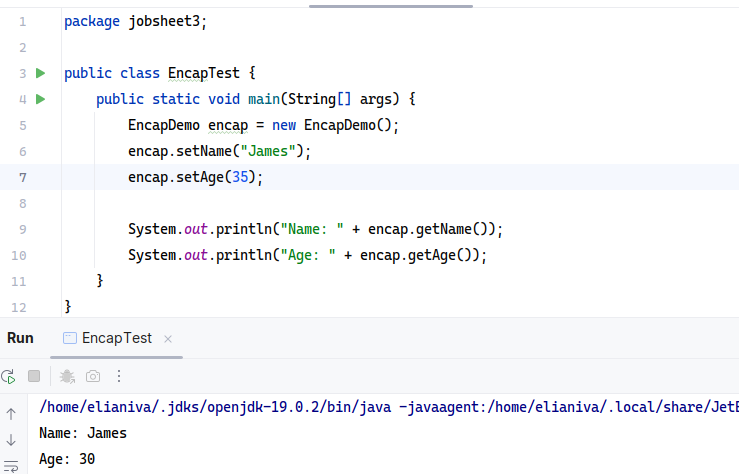
\includegraphics[width=.8\textwidth]{./images/task-1.png}
        \end{center}
    }
    \item {
        On the program above, we've set the age to be 35 but we got 30. Explain why!

        Because we've capped the max age to be 30 on the setter. Any value above 30 will be set to 30
        by the setter \texttt{setAge(int age)}.
    }
    \item {
        Change the program above so that it has a minimum age of 18 and a maximum age of 30!

        \begin{minted}[fontsize=\small,autogobble]{java}
            public void setAge(int newAge) {
                if (newAge > 30) {
                    age = 30;
                } else if (newAge < 18) {
                    age = 18;
                } else {
                    age = newAge;
                }
            }
        \end{minted}
    }
    \item {
        \begin{minted}[fontsize=\small,autogobble]{java}
            public class Anggota {
                public String nomorKTP;
                public String nama;
                public int limitPinjaman;
                public int jumlahPinjaman;

                public Anggota(String nomorKTP, String nama, int limitPinjaman) {
                    this.nomorKTP = nomorKTP;
                    this.nama = nama;
                    this.limitPinjaman = limitPinjaman;
                }

                public String getNama() {
                    return nama;
                }

                public int getLimitPinjaman() {
                    return limitPinjaman;
                }

                public int getJumlahPinjaman() {
                    return jumlahPinjaman;
                }

                public void pinjam(int pinjam) {
                    if (pinjam > limitPinjaman) {
                        System.out.println("Maaf, jumlah pinjaman melebihi limit.");
                    } else {
                        jumlahPinjaman += pinjam;
                    }
                }

                public void angsur(int pinjam) {
                    jumlahPinjaman -= pinjam;
                }
            }
        \end{minted}
    }
    \item {
        Modify so that the amount of the minimum installments is 10\% of the loan amount!
        If the amount of the installments is less than 10\% of the loan amount, then show
        a warning message "Sorry, the installment amount is less than 10\% of the loan amount".

        \begin{minted}[fontsize=\small,autogobble]{java}
            public void angsur(int pinjam) {
                if (pinjam < (jumlahPinjaman * 0.1)) {
                    System.out.println("Maaf, angsuran harus 10% dari jumlah pinjaman.");
                } else {
                    jumlahPinjaman -= pinjam;
                }
            }
        \end{minted}
    }
    \pagebreak
    \item {
        Modify the class \texttt{TestKoperasi} so that it can retrieve the amount of the loan
        and the amount of the installments from user input!

        \begin{minted}[fontsize=\small,autogobble]{java}
            public class TestKoperasi {
                public static void main(String[] args) {
                    Scanner scanner = new Scanner(System.in);
                    Anggota donny = new Anggota("111333444", "Donny", 5000000);
                    System.out.println("Nama Anggota: " + donny.getNama());
                    System.out.println("Limit Pinjaman: " + donny.getLimitPinjaman());

                    System.out.print("Masukkan jumlah pinjaman: ");
                    int pinjam = scanner.nextInt();
                    donny.pinjam(pinjam);
                    System.out.println("Jumlah pinjaman saat ini: " + donny.getJumlahPinjaman());

                    System.out.print("Masukkan jumlah angsuran: ");
                    int angsur = scanner.nextInt();
                    donny.angsur(angsur);
                    System.out.println("Jumlah pinjaman saat ini: " + donny.getJumlahPinjaman());

                    System.out.print("Masukkan jumlah angsuran: ");
                    angsur = scanner.nextInt();
                    donny.angsur(angsur);
                    System.out.println("Jumlah pinjaman saat ini: " + donny.getJumlahPinjaman());
                }
            }
        \end{minted}

        \begin{center}
            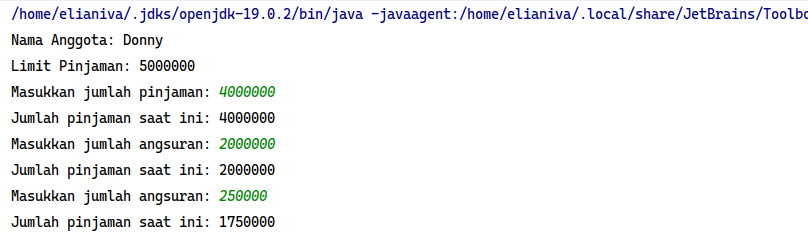
\includegraphics[width=.8\textwidth]{./images/task-2.png}
        \end{center}
    }
\end{enumerate}

\end{document}

